\begin{apendicesenv}
	% Imprime uma página indicando o início dos apêndices
	\partapendices
	\begin{landscape}
		\chapter{Aplicação de um filtro \textit{Wavelet}}
		\begin{figure}[h]
			\caption{Demostração numérica das transformadas Wavelet e \textit{packet-wavelet}: Por razões didáticas a \textit{Wavelet} Haar foi considerada como tendo os valores $1/2$ e $-1/2$}
			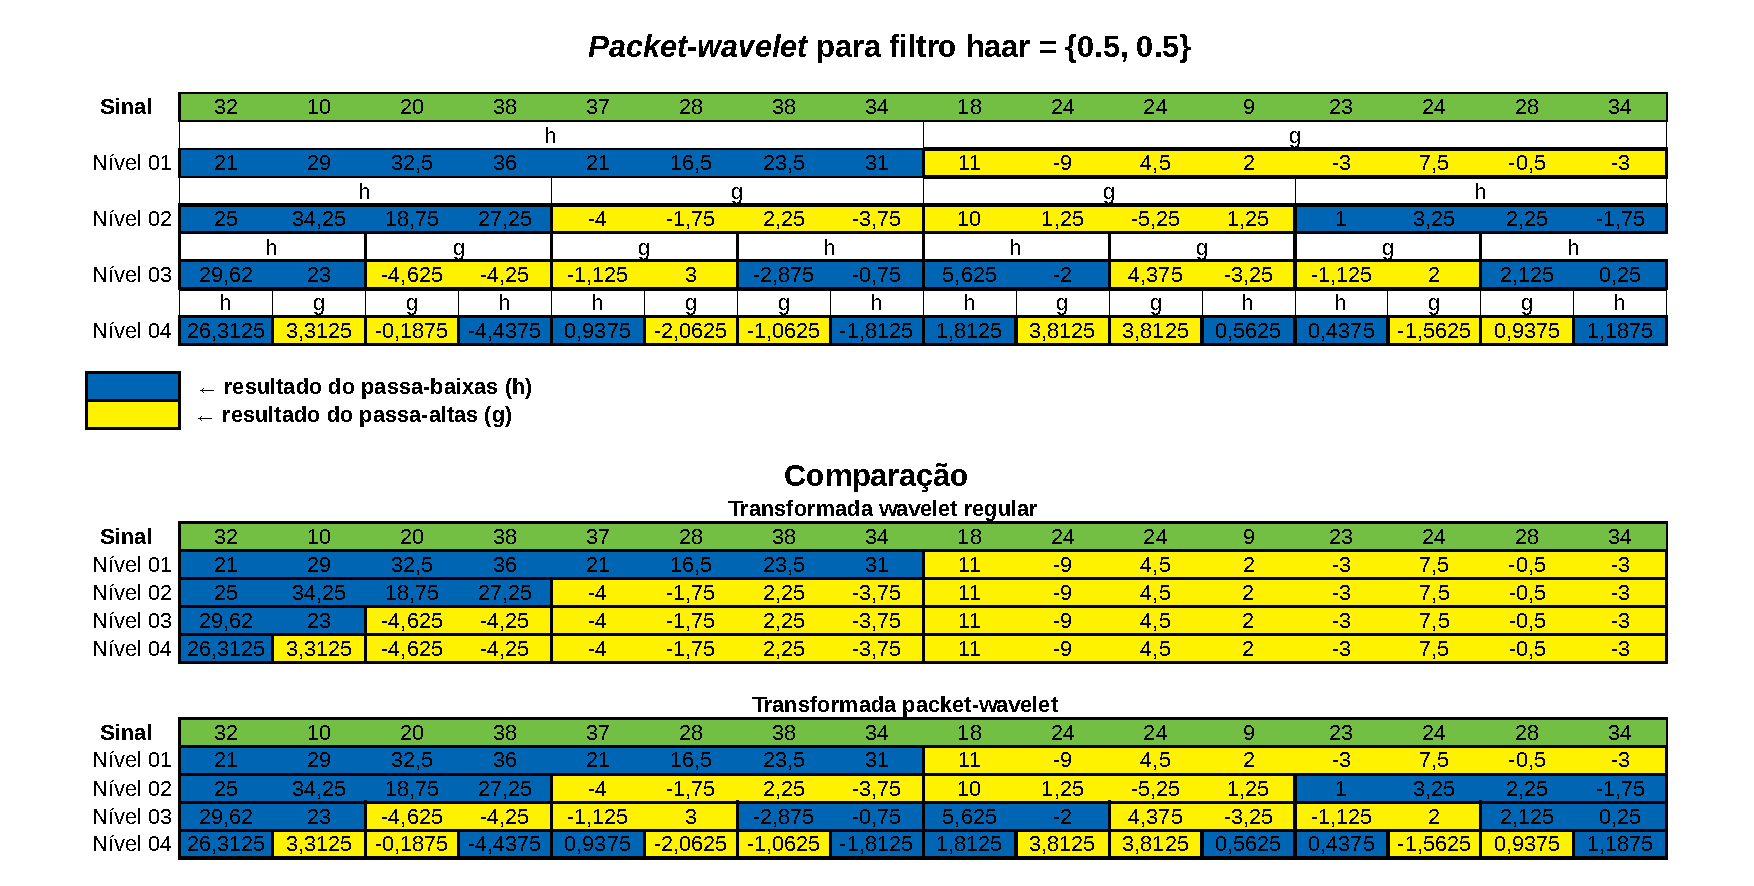
\includegraphics[width=.93\linewidth]{images/haarWaveletExamples.pdf}
			\label{fig:haarWaveletExamples}
			\\Fonte: Elaborado pelo autor, 2021.
			
		\end{figure}
	\end{landscape}

	\chapter{Arquivos digitais \textit{wave}}
		\label{chap:waveFile}
		\par Os arquivos no formato digital \textit{wave}, popularmente utilizados para armazenar áudio e voz digital \cite{WAVE2019}, assim como ocorre neste trabalho, se estruturam como ilustrado na Figura \ref{fig:wavePcmStructure}.
		
		\begin{figure}[h]
			\centering
			\caption{Estrutura do arquivo Wave}
			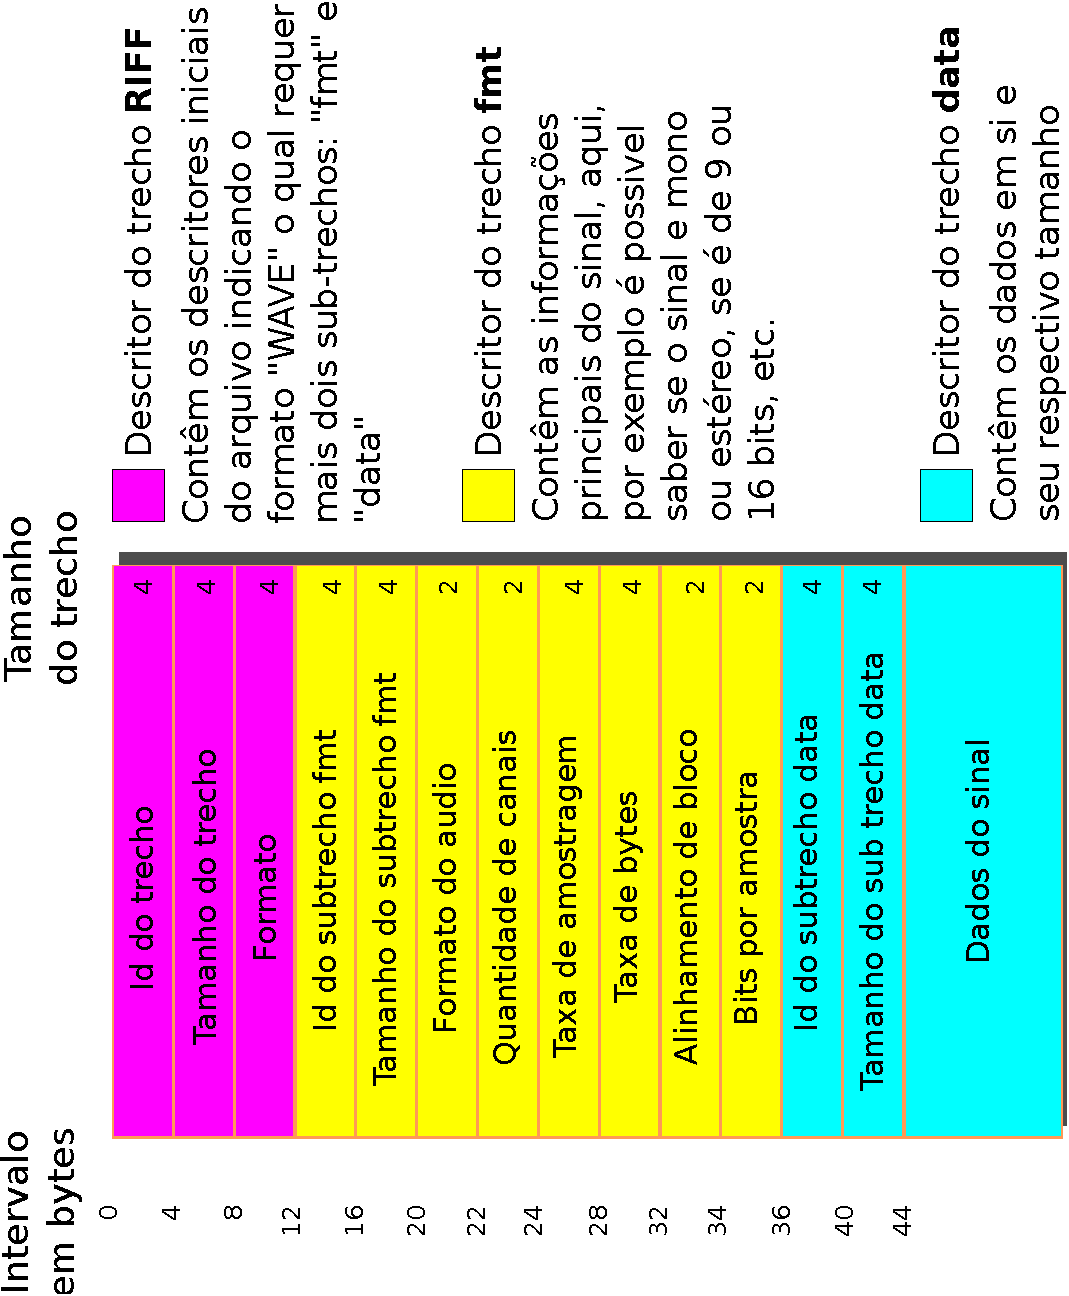
\includegraphics[width=0.6\linewidth, angle=-90]{images/wavePcmStructure.pdf}
			\label{fig:wavePcmStructure}
			\\Fonte: Elaborado pelo autor, 2021.
		\end{figure}
		
		\par A estrutura de interesse se localiza na última parte do arquivo, mais especificamente no bloco ``data'' ilustrado em azul na Figura. Nele, os dados são organizados como um grande vetor de números, em formato \textit{little endian} \cite{adiga2007writing}, sendo que cada um deles indica a intensidade do sinal naquele ponto. A descrição pormenorizada do bloco ``data'', consultada em \cite{microsoftIbmWaveSpec}, foi utilizada neste trabalho para possibilitar a extração dos dados brutos dos sinais utilizados. 

	\chapter{Recursos na web}
		\par Para realização deste trabalho foram produzidos variados textos (este incluso) e códigos, é recomendada a consulta dos códigos fontes utilizados nos procedimentos como complemento que, se espera, melhore o entendimento dos assuntos discutidos.
		
		\par Uma atenção especial deve ser dada ao diretório localizado em \textit{\textbf{/src/lib}} que contém todas as bibliotecas criadas e referenciadas para resolver os problemas surgidos e também ao \textit{\textbf{/src/experiments}} que contém os procedimentos já descritos.
				
		\par Em \textit{\textbf{/soundSamples}} se encontra a base de dados com os áudios originais e tratados.
		
		\par Alguns \textit{scripts} foram desenvolvidos para facilitar o tratamento dos arquivos de áudio, os mesmos se encontram em \textbf{\textit{/src/scripts}}.
		
		\par Por fim a parte escrita pode ser consultada em \textit{\textbf{/documentation}}.
		
		\par Todos esses materiais estão sob licença de código aberto (GPLv3) e são livres para uso não comercial acesse   \href{https://github.com/ensismoebius/voiceSpoofingDetectionWavelet}{https://github.com/ensismoebius/voiceSpoofingDetectionWavelet} para mais informações.
\end{apendicesenv}